\section{TO DO Items}

\begin{itemize}
\item Add destructive object-field-update \emph{x.f := y} to the language.
\item Add if-then-else to the language.
\item Omit constructors from classes (and use an implicit constructor).
\item Note that the claim that all region variables will be unified with some concrete
region fails in the case of a method that recursively calls itself (and, hence, does not
terminate). In this case, the region variables in the return type are not constrained.
Similarly for non-terminating mutual recursion. These are uninteresting (in essence, the
return type can be taken to be unit instead).
\item Discuss the safety of virtual method invocation, which provides a limited form
of existentially quantifying regions and instantiating (unpacking) them because a
derived class may have more region parameters than a base class.
\item Discuss the subtyping rule used to check an overriding method (in the static
semantics).
\item Mention that constraints are in the theory of partial orders?
\end{itemize}

\section{Type Inference}
\label{sec:type-inference}

\name's region type system imposes a heavy annotation burden, and
manually annotating C\# standard libraries with region types
can be tedious. We now present our region type inference algorithm
that eliminates the need to write region type annotations.
% except on some higher-order functions.
Formally, the type inference
algorithm is an elaboration function from programs in $\absof{\FB}$
(i.e., \FB without region types, but with \C{letregion} and \C{open}
expressions, similar to the language introduced in
\S~\ref{sec:overview}) to programs in \FB.

\paragraph{Overview.}
In the sequel, we will be using \emph{region identifiers} in four different roles.
A region identifier may serve as
(a) A \emph{formal region parameter} of a class or method, or
(b) a \emph{static region identifier} introduced by a \C{letregion} construct, or
(c) an  \emph{open transferable region identifier} introduced by an \C{open} construct, or
(d) a \emph{region variable}, introduced to represent an unknown actual region parameter
of a method invocation or object alloation,
which will be bound to a region identifier of one of the three
preceding kinds by the end of the type inference.

Fig.~\ref{fig:type-inference-algo} presents the high-level outline of the type
inference algorithm.
The algorithm consists of the following steps:
\begin{enumerate}
 \item \emph{Region Parametrization}.
   The first step elaborates the input program by introducing \emph{formal region parameters}
   (for each class and method), and \emph{region variables} (representing yet undetermined
   \emph{actual region parameters}). We also introduce for each class and method, a
   \emph{predicate variable} ($\varphi$) to denote an undetermined set of constraints
   over the region parameters of that class/method.

%%    as follows:
%% \begin{enumerate}
%% \item For every class determine a set of \emph{region parameters} ($\rho$)
%%        it should be parametrized over.
%% \item For every field of the class, determine its region parametrized type by
%%        generating as many fresh \emph{actual region parameters} as required by its class (type),
%%        which in turn become formal region parameters of the containing class.
%% \item  For every method and function type, determine its corresponding region
%%    type template by introducing fresh region parameters as required by
%%    the type of each parameter and return value (in addition to the allocation region
%%    parameter).
%%  \item Elaborate every \C{new} expression, method call or function application by
%%    introducing \emph{fresh region variables} (as required by the region type
%%    template of the called method or function).
%% \item Introduce for each class and method, a \emph{predicate variable} ($\varphi$) to denote
%%    an undetermined set of constraints over the region parameters of that
%%    class/method.
%% \end{enumerate}

 \item \emph{Constraint Generation}.
   In the second step, we analyze the program to generate a set of constraints
   (over the region identifiers and the predicate variables)
   that must hold (as per the static semantics in Fig.~\ref{fig:fb-staticsem}).

 \item \emph{Constraint Solving}.
   We solve the generated set of constraints using our fixpoint constraint
   solving algorithm \csolvestar, which reduces the constraint solving problem to
   an abduction problem. If the original program in $\absof{\FB}$ contains unsafe
   references, for example, a reference from a transferable region to a
   stack region, then the constraints generated during the elaboration
   are not satisfiable. In such a case, \csolvestar{} fails to solve
   the constraints.
% in a Herbrand constraint system, and then relies on \csolve,
% our abduction solver for that domain. 

 \item If the solver succeeds, it returns substitution functions $\substFn_\rho$ and
  $\substFn_\varphi$ for free region and predicate variables, respectively, introduced in
  step 1. We apply these substitutions to the elaborated program to produce the final program.


\end{enumerate}



\begin{figure}
\begin{numcodeml}
Infer ($p$) =
  let $q$ = IntroduceRegionParameters($p$) in
  let $(r,C)$ = GenerateConstraints($q$) in
  match (SolveConstraints($C$) with
  | None $\longrightarrow$ None
  | Some ($s$) $\longrightarrow$ Some (ApplySolution $(s,r)$)
\end{numcodeml}

\caption{The type inference algorithm}
\label{fig:type-inference-algo}
\end{figure}

\begin{theorem}
\emph{(\textbf{Soundness})}
For any $p \in \absof{\FB}$, if Infer($p$) returns Some($t$), then
(1) $\absof{t} = p$, and
(2) $t$ is well-typed.
\end{theorem}



%%    This is used to replace every FGJ type in the program
%%    compute a polymorphic region type template
%%     for every class and method from their FGJ types. The templates contain
%%     region variables ($\rho$) to denote unknown region annotations, and
%%     predicate variables ($\varphi$) to denote unknown constraints over
%%     such region annotations. Free region variables are generalized in these
%%     types (which are, hence, polymorphic).
%%  
%%    Second, we make use of the computed region type templates to elaborate
%% expressions by introducing region variables to denote unknown region
%% arguments in \C{new} expressions, method calls and function
%% applications.
%% While elaborating expressions, we also build a system of
%% constraints that capture well-formedness requirements and subtyping
%% relationships between type templates that must hold (as per the static
%% semantics in Fig.~\ref{fb-staticsem}) for the elaboration to be valid.
%% Third, we lift expression elaboration and constraint generation to
%% methods and classes. Finally, we solve the constraints by making use
%% of our fixpoint constraint solving algorithm \csolvestar, which
%% reduces the constraint solving problem to an abduction problem in a
%% Herbrand constraint system, and then relies on \csolve, our abduction
%% solver for that domain. 

% Due to the presence of region-polymorphic
% recursion in \FB, constraints generated by the algorithm can be
% circular. More precisely, constraints generated can assume the form
% $\varphi \Leftrightarrow \phi \wedge F(\varphi)$, where $F$ is a
% non-idempotent substitution function for region variables in
% $\varphi$. In the constraint solving phase, the algorithm then relies
% on a fixpoint constraint solving algorithm called \csolvestar to solve
% the constraints and determine assignments for unknown region and
% predicate variables.

\subsection{Region Parametrization/Instantiation for Classes}
\label{sec:fb-templatization}

The first phase is an iterative process involving the following three steps,
the first two of which are mutually dependent on each other.

\emph{Region Parametrization}. For every class \C{C}, we identify
a sequence of formal region parameters $\pi_0, \cdots \pi_n$ that \C{C}
should be parametric over.

\emph{Parameter Instantiation}.
We then replace every instance of class \C{C} in the program by an instance
$\C{C}\langle \rho_0, \cdots, \rho_n \rangle$, where $\rho_0, \cdots, \rho_n$
are fresh identifiers denoting actual region parameters.

\emph{Predicate Variable Introduction}. For every class \C{C}, we introduce
a fresh predicate variable $\varphi$, which represents the yet undetermined
outlives constraints between the formal region parameters of class \C{C}.

We identify the region parameters of classes as follows.

\emph{Non-Recursive Classes}.
The class \C{Object} is defined to have a single region parameter $\pi_0$ (the allocation region).
The region parameters for any other non-recursive class \C{C} is determined
only after the region parameters of any class that \C{C} depends on have been
determined: this includes the base-class \C{B} of \C{C} and the class (type)
of any of its fields.
We replace every dependee type \C{T} in \C{C} by its instantiated type,
using fresh region parameters as needed.
The sequence of region parameters for \C{C} is defined to be
the sequence of region parameters for the base class \C{B} concatenated
with the list of all  fresh region parameters introduced while instantiating the types
of the fields in the class.
(The class inherits its allocation region from its base class. Note that if
a class does not specify an explicit base class, it has an implicit base class
\C{Object}.)

This transformation is illustrated below, using a non-generic \C{Pair} class:

\begin{tabular}{ccc}
\begin{minipage}{0.28\linewidth}
\begin{codejava}
class Pair
  $\extends$ $\ObjZ$
{
  $\ObjZ$ fst;
  $\ObjZ$ snd;
}
\end{codejava}
\end{minipage}
&
$\Rightarrow$
&
\begin{minipage}{0.5\linewidth}
\begin{codejava}
class Pair $\langle \rho_0, \rho_1, \rho_2 \; | \; \varphi \rangle$
  $\extends$ $\ObjZ \langle \rho_0 \rangle$
{
  $\ObjZ \langle \rho_1 \rangle$ fst;
  $\ObjZ \langle \rho_2 \rangle$ snd;
}
\end{codejava}
\end{minipage}
\end{tabular}

\emph{Recursive Classes}.
The region parameters for a recursive class is computed in
a similar fashion, with the following difference: any recursive
field is ignored while instantiating region parameters for the fields of
the class, and the region parameters of the recursive class are computed
as before. We then do parameter instantiation for all recursive fields,
such that their region annotations (the actial region parameters) are
exactly the same as the (formal) region parameters of the class.
The following example illustrates this for a non-generic \C{List} class.
The resulting class represents a linked list with spine in the region
$\rho_0$ and data objects in the region $\rho_1$.

\begin{tabular}{ccc}
\begin{minipage}{0.28\linewidth}
\begin{codejava}
class List
  $\extends$ $\ObjZ$
{
  $\ObjZ$ data;
  List next;
}
\end{codejava}
\end{minipage}
&
$\Rightarrow$
&
\begin{minipage}{0.5\linewidth}
\begin{codejava}
class List $\langle \rho_0, \rho_1 \; | \; \varphi \rangle$
  $\extends$ $\ObjZ \langle \rho_0 \rangle$
{
  $\ObjZ \langle \rho_1 \rangle$ data;
  List $\langle \rho_0, \rho_1 \rangle$ next;
}
\end{codejava}
\end{minipage}
\end{tabular}

The above technique can be extended to mutually recursive classes in a
straightforward manner, by simultaneously parametrizing them (and
then instantiating them).

\emph{Type-Parametric Classes}.
The techniques described above can be used for parametrized classes
with the following extension. Consider a parametrized class \C{C $\langle$ T $\extends$ B $\rangle$}.
The parametric type \C{T} is instantiated using the number of region parameters
that its bound \C{B} has. If no bound is specified for \C{T}, the bound is taken
to be \C{Object}, and \C{T} is instantiated with one region parameter.

\emph{Function Types}.
Since \FB{} is higher-order, fields of function type are allowed. The parameter instantiation step
instantiates function types as follows: the type of every parameter as well as the return value is
instantiated with fresh region identifiers, as described earlier, and finally these region identifiers
are generalized as formal region parameters of the function type.
For example, the function type $\C{List} \rightarrow \C{Object}$ is instantiated as
$\inang{\rho_0, \rho_1, \rho_2} \C{List} \inang{\rho_0,\rho_1} \rightarrow \C{Object}\inang{\rho_2}$.

%% Likewise, given the region-annotated definition of
%% \C{Pair} class from \S\ref{sec:fb-syntax} a region type template for a
%% method with FGJ type $\C{Pair}\inang{\C{A},\C{B}} \rightarrow \C{A}$
%% is \footnote{In our exposition, we assume that classes $\C{A}$ and
%% $\C{B}$ are trivial subclasses of $\ObjZ$ with no fields/methods. Like
%% $\ObjZ$, they accept one region parameter - the allocation region of
%% their objects.}\footnote{We abuse arrow notation to also represent
%% types of methods, but unlike function types, there is no allocation
%% region annotation atop the arrow in a method type.}
%% $\inang{\rhoalloc_0,\rho_1,\rho_2,\rho_3 \,|\, \varphi_0}
%% \C{Pair}\inang{\C{A},\C{B}} \inang{\rho_1,\rho_2,\rho_3} \rightarrow
%% \unitZ$, where $\rhoalloc_0$ and $\rho_{1-3}$ are fresh region
%% variables, and $\varphi_0$ is a fresh predicate variable denoting
%% unknown constraints over $\rhoalloc_0$ and $\rho_{1-3}$.

\subsection{Region Parametrization/Instantiation for Methods}

As the next step, we introduce region parameters for every method.
We do this by instantiating the types of all parameters and the
return value (of the method) using fresh region identifiers (as explained previously),
and then generalizing these region identifiers as formal region parameters
of the method. As for the classes, we also introduce a fresh predicate variable
$\varphi$ for every method.

We then consider every method invocation in the program, and introduce
fresh region variables representing the (yet unknown) actual region
parameters for this particular invocation.
%
We similarly perform instantiation for every constructor invocation
of the form \C{new T($\ldots$)}, by instantiating the type \C{T} as
before, turning it into \C{new T$\langle \rho_0, \cdots, \rho_n \rangle$($\ldots$)},
where $\rho_0, \cdots, \rho_n$ are fresh region variables.

\subsection{Constraints}
\label{sec:fb-constraintsem}

% mathpartir's inferrule: seems to have problems with linebreaks
\newcommand{\genconstraint}[2]{\inferrule*{#1}{#2}}
\newcommand{\gcarrow}{\leadsto}
\newcommand{\gctransforms}{\models}

\newcommand{\gcrule}[2]{%
\begin{smathpar}\begin{array}{c}%
\renewcommand*{\arraystretch}{1.2}%
\RULE {#1} {#2}%
\end{array}\end{smathpar}%
}

\newcommand{\minigcrule}[3]{%
\begin{minipage}{#1}\begin{smathpar}\begin{array}{c}%
\renewcommand*{\arraystretch}{1.2}%
\RULE {#2} {#3}%
\end{array}\end{smathpar}\end{minipage}%
}

\newcommand{\subtypesym}{<:}

\newcommand{\typeok}[3]{{#1\,\vdash\,#2 \; \texttt{ok} \, \lhd #3}}
\newcommand{\exprok}[4]{{#1} \, \vdash \, {#2} : {#3} \, \lhd {#4}}
\newcommand{\subtypeok}[4]{{#1} \, \vdash \, {#2}  \subtypesym {#3} \, \lhd {#4}} 

\newcommand{\stdcontext}{\exptycx{\ralloc}{\env}}

\begin{figure*}[t]
% \begin{mathpar}

% NEW
  \gcrule
  {
    \typeok {\A} {\fbN} {C_1} \spc
    \exprok {\stdcontext} {\bar{e}} {\bar{\tau'}} {C_2} \spc
    C_3 = \{ \isvalid{\A.\phicx}{\allocRgn(\fbN)=\ralloc} \} \spc
    \fields(\fbN) = \bar{f} : \taubar \spc
    \subtypeok {\A} {\bar{\tau'}} {\bar{\tau}} {C_4}
  }
  {
    \exprok {\stdcontext}   {\C{new} \fbN(\bar{e})} {\fbN} {\cup_{i=1}^4 C_i}
  }

% FUNCTION INVOCATION
\gcrule
{
\exprok {\stdcontext} {e_a} {\inang{\rho_0 \rhobar\,|\,\phi}\taubar \xrightarrow{\rgn} \tau} {C_1} \spc
\exprok {\stdcontext} {\bar{e}} {\bar{\tau'}} {C_2} \spc
\substFn = [\bar{\rho'}/\rhobar][\rho_0'/\rho_0]
\\
C_3 = \{\rho_0' \bar{\rho'} \in \A.\rhoenv\} \spc
C_4 = \{\isvalid{\A.\phicx}{\substFn(\phi)}\} \spc
\subtypeok {\A} {\bar{\tau'}} {\substFn(\bar{tau})} {C_5}
}{
\exprok {\stdcontext} {e_a\inang{\rho_0'\bar{\rho'}}(\bar{e})} {\tau} {\cup_{i=1}^5 C_i}
}

% Original from elaboration algorithm:
% $e_a(\bar{e})$ $\longrightarrow$ 
%    let ($e_a':\inang{\rhoalloc\rhobar\,|\,\phi}\taubar \xrightarrow{\rgn} \tau$,$C_1$) = 
%                $\elabExpr(\A,\ralloc,\env,e_a)$ in
%    let $\bar{\rho'}$ = $\bar{\fresh_\rho()}$ in
%    let $C_2$ = $\{\bar{\rho'} \in \A.\rhoenv\}$ in
%    let $\substFn$ = $[\bar{\rho'}/\rhobar][\ralloc/\rhoalloc]$ in
%    let $C_3$ = $\{\isvalid{\A.\phicx}{\substFn(\phi)}\}$ in
%%*   %let $(C_3,C_4)$ = $(\typeOk(\substFn(\taubar)), \typeOk(\substFn(\tau)))$ in 
%*)   let $(\bar{e'}:\bar{\tau'}, C_4)$ = $\elabExpr(\A,\ralloc,\env,\bar{e})$ in
%    let $C_5$ = $\subtypeOk({\A},{\bar{\tau'}},{\bar{\substFn(\tau)}})$ in
%      ($e_a'\inang{\ralloc\bar{\rho'}}(\bar{e'}):\substFn(\tau)$,$\bigcup_{i=1}^5 C_i$)

% LET-REGION
\gcrule{
\A= (\rhoenv,\aenv,\phicx)  \spc
\rgn \notin \rhoenv \spc
\A' = (\rhoenv \cup \{\rgn\}, \aenv, \phicx \conj (\rhoenv \outlives \rgn))  \spc
\exprok{\A',\rgn,\env} {e_a} {\tau} {C_1} \spc
\typeok {\A} {\tau} {C_2}
}{
\exprok{\stdcontext} {\letregion{\rgn}{e_a}} {\tau} {(C_1 \cup C_2)}
}

% Original from elaboration algorithm:
%  | $\letregion{\rgn}{e_a}$ $\longrightarrow$
%    let $\rgn'$ = $\fresh_{\rgn}()$ in 
%    let $(\rhoenv,\aenv,\phicx)$ = $\A$ in
%    let $\A'$ = ($\rhoenv \cup \{\rgn'\}, \aenv, \phicx \conj (\rhoenv \outlives \rgn')$) in
%    let ($e_a':\tau$,$C_1$) = $\elabExpr(\A',\rgn',\env,[\rgn'/\rgn]e_a)$ in
%      ($\letregion{\rgn'}{e_a'}:\tau$,$C_1$)

\gcrule{
\exprok {\stdcontext} {e_a} {\RgnZ\inang{T}\inang{\rho}} {C_1} \spc
\A = (\rhoenv,\aenv,\phicx) \spc
\rgn \notin \rhoenv \spc
(\A',\env') = ((\rhoenv \cup \{\rgn\},\aenv,\phicx),\env[y\mapsto T@\rgn] \spc
\exprok {\A',\rgn,\env'} {e_b} {\tau} {C_2}
}{
\exprok {\stdcontext} {\open{e_a}{\rgn}{y}{e_b}} {\tau} {C_1 \cup C_2}
}

% Original from elaboration algorithm:
%  | $\open{e_a}{\rgn}{y}{e_b}$ $\longrightarrow$ 
%    let ($e_a':\RgnZ\inang{T}\inang{\rho}$,$C_1$) = 
%                $\elabExpr(\A,\ralloc,\env,e_a)$ in
%    let $\rgn'$ = $\fresh_{\rgn}()$ in 
%    let $(\rhoenv,\aenv,\phicx)$ = $\A$ in
%    let ($\A'$,$\env'$) = ($(\rhoenv \cup \{\rgn'\},\aenv,\phicx)$,$\env[y\mapsto T@\rgn']$) in
%    let ($e_b':\tau$,$C_2$) = $\elabExpr(\A',\rgn',\env',[\rgn'/\rgn]e_a)$ in
%      ($\open{e_a'}{\rgn'}{y}{e_b'} : \tau$, $C_1 \cup C_2$)



% \end{mathpar}
\caption{Constraint generation}
\label{fig:constraint-gen}
\end{figure*}


%Fresh predicate variable $\varphi_0$ denotes unknown constraints over
%$\rhoalloc_0$ and $\rho_{0-4}$ that need to hold for template to be a
%well-formed region-annotated class definition in $\FB$. 

The constraint generation algorithm mimics the static type checker, but accumulates
constraints that must hold for the type checking to succeed.

\emph{Class Constraints}. 
Computing the class constraint $\varphi_{\C{C}}$ corresponding to a class \C{C} is
fairly straightforward. It is the conjunction of
\begin{itemize}
\item $\conj_{1 \leq i \leq n} (\rho_i \outlives \rho_0)$
\item $\varphi_{\C{B}}$
\item $[\rho_a/\rho_f]\varphi_{\C{F}}$
\end{itemize}

Our constraint generation algorithm generates the following kinds of constraints:
\begin{itemize}
\item Well-formedness constraints of form $\rho \in \rhoenv$,
restricting the domain of unification for a region variable ($\rho$)
to the set ($\rhoenv$) of regions in scope,
\item Well-formedness constraints of form
$\tywf{\rhoenv}{\varphi}$, restricting the domain of a predicate
variable ($\varphi$) to the set of all possible constraint formulas
over region variables ($\rhoenv$) in scope, and
\item Validity constraints of form $\isvalid{\phictxt \conj \varphi_i} {\phicstr}$
where $\varphi_i$ is a predicate variable (representing the precondition of a
method to be determined), $\phicstr$ is a region constraint that is \emph{required}
to hold at a particular program point (within the method), and $\phictxt$ is
a region constraint that is \emph{known} to hold at that program point.
Each $\phi$ is a region constraint over region variables and region parameters:
\begin{smathpar}
\begin{array}{lcl}
\phi & \coloneqq & true \ALT \rho \outlives \rho \ALT \rho = \rho \ALT \phi \conj \phi \\
\end{array}
\end{smathpar}
%
%% Formulas $\phictxt$ and $\phicstr$ are concrete, i.e., free
%% of predicate variables and pending substitutions. While $\phictxt$
%% captures relationships that are \emph{known} to hold between concrete
%% region identifiers (i.e., $\rgn$'s) when the constraint was generated,
%% $\phicstr$ captures relationships that are \emph{required} to hold
%% among region varibles (i.e., $\rho$'s), or relationships between
%% region variables and identifiers.
%
\item Validity constraints of the form $\isvalid{\phictxt \conj \varphi_i} {F_j(\varphi_j)}$
generated by an invocation of a method with precondition $\varphi_j$ (where $\phictxt$ and
$\varphi_i$ are as above).
Here, $F$ denotes \emph{pending substitutions}\footnote{we borrowed this terminology from~\cite{ltpldi08}}:
it serves to bind formal region parameters in $\varphi_j$ to the actual region parameters
at a particular invocation site.
\begin{smathpar}
\begin{array}{lcl}
F & \coloneqq & \cdot \ALT [\rho/\rho]F \\
\end{array}
\end{smathpar}
\end{itemize}

A pending substitution ($F$) is a substitution function over region
variables/identifiers. They represent the substitutions that need to
be carried out when a predicate variable ($\varphi$) is replaced by a
concrete formula in a validity constraint. For instance, in the
validity constraint $\isvalid{\rgn_1 \outlives
\rgn_2}{[\rgn_1/\rho_1][\rgn_2/\rho_2]\varphi}$, pending substitution
is $[\rgn_1/\rho_1][\rgn_2/\rho_2]$. Any concrete formula (call it
$\phisol$) over variables $\rho_1$ and $\rho_2$ is a solution to
$\varphi$ if and only the formula obtained by substituting $\rgn_1$
and $\rgn_2$ for $\rho_1$ and $\rho_2$ (resp.) in $\phisol$ is
deducible from $\rgn_1 \outlives \rgn_2$.

% Validity constraints primarily result from checking if a region type
% template of form $B\inang{\tbar}\inang{\rhoalloc,\rhobar}$ is
% well-formed (i.e., $\typeOk$). The corresponding well-formedness rule
% (Fig.~\ref{fig:fb-staticsem}) requires that the instantiation of $B$'s
% formal region parameters with actual region arguments satisfy its
% precondition, where actuals are subsituted for formals. Since $B$'s
% precondition could be unknown, the requirement results in a in a
% validity constraint with predicate variables and pending
% substitutions. Other sources of validity constraints are calls to
% region-polymorphic methods, where similar situation arises. 

%
%% If the constraint is generated while checking the well-formedness of a
%% type or elaborating an expression, then $\varphi_j$'s denote the unknown
%% preconditions of classes and methods that were used in that type or expression.
%
% Each use of a (region-polymorphic) class or a method may instantiate region
% parameters differently, resulting in a different pending substitution
% ($F_j$).

Each region variable occuring in $\phicstr$ has an associated well-formedness
constraint, which specifies its unification domain. The unification domain of a
constraint is the union of unification domains of all region variables
occuring in the constraint.

\paragraph{Constraints Example 1} Consider the $\C{Pair}$ class
template from \S\ref{sec:fb-templatization}. Following constraints are
generated during its elaboration (Constrains are identified with
$\mathbf{c_i}$'s. Some trivial constraints, such as $\rho_4 \in
\rhoenv_0$ and $\rho_5 \in \rhoenv_1$, where $\rhoenv_0 =
\{\rhoalloc_0,\rho_{0-4}\}$ and $\rhoenv_1 = \rhoenv_0 \cup
\{\rho_5\}$, have been elided): 
\begin{smathpar}
\begin{array}{l}
  \csid{1} \tywf{\rhoenv_0}{\varphi_0} \qquad
  \csid{2} \isvalid{\varphi_0}{\rho_0 \outlives \rhoalloc_0 \conj \rho_1
     \succeq \rhoalloc_0 \conj \rho_4 = \rhoalloc_0} \\
  \csid{3} \isvalid{\varphi_0}{\rho_2 = \rho_0} \spc
  \csid{4} \isvalid{\varphi_0}{\rho_3 = \rho_1} \\
  \csid{5} \isvalid{\varphi_0 \conj \varphi_1} {\rho_5 = \rho_0}\spc
  \csid{6} \tywf{\rhoenv_1}{\varphi_1} \qquad
\end{array}
\end{smathpar}

\paragraph{Constraints Example 2} Let us add to the \C{Pair} class a
contrived method $\C{alt}$ that accepts a \C{Region} object \C{r}, a
\C{Pair<A,A>} object \C{q}, and an \C{A} object \C{y}. It assigns
\C{y} to \C{fst} and \C{snd} fields of \C{q}, and calls itself
recursively with the same region, a new \C{Pair} object allocated in a
local region, and an \C{A} object referred by the \C{snd} field of the
pair inside the region. \C{alt} never terminates.  Elaboration phase
elaborates the method to the following region-annotated
definition\footnote{In reality, elaboration uses new region variables
as parameters to the constructor and method calls, and then generates
constraints that unify them with actuals. In our examples, to avoid
clutter due to trivial constraints,we coalesced both steps and show
the actuals instead.}(The original definition of \C{alt} can be
obtained by erasing all the region annotations from the elaborated
version):
% \begin{codejava}
% unit alt<$\rhoalloc_2$,$\rho_{6-10}$ | $\varphi_2$>(Pair<A,A><$\rho_6$,$\rho_7$,$\rho_8$> p,
%                           A<$\rho_9$> x, A<$\rho_{10}$> y) {
%   p.fst = x; p.snd = y; 
%   this.alt<$\rhoalloc_2$,$\rho_7$,$\rho_8$,$\rho_{10}$,$\rho_9$>(A,y,x);
% }
% \end{codejava}
\begin{codejava}
unit alt<$\rhoalloc_2$,$\rho_{6-9}\,$|$\,\varphi_2$>(Region<Pair<A,A>><$\toprgn$> r, 
                Pair<A,A><$\rho_{6-8}$> q, A<$\rho_{9}$> y) {
  q.fst := y; q.snd := y; 
  open r as p@$\rgn_0$ in
    letregion $\rgn_1$ in
      let x = new Pair<A,A><$\rgn_1$,$\rgn_0$,$\rgn_0$>
                      (p.fst,p.fst) in
        alt<$\rgn_{1}$,$\rgn_{1}$,$\rgn_{0}$,$\rgn_{0}$,$\rgn_{0}$>(r,x,p.snd)
}
\end{codejava}
% Note that, to avoid clutter, we have already resolved appropriate
% region arguments to the recursive call, instead of introducing new
% region variables and generating equality constraints on them. 
Constraints generated during the elaboration are shown below
(let $\rhoenv_2 = \{\rhoalloc_0,\rho_{0-4},\rhoalloc_2,\rho_{6-9}\}$ ):
\begin{smathpar}
\begin{array}{l}
\csid{7} \tywf{\rhoenv_2}{\varphi_2}\qquad
\csid{8} \isvalid{\varphi_1 \conj \varphi_2}
    {\rho_7 \outlives \rho_6 \conj \rho_8 \outlives \rho_6} \\
\csid{9} \isvalid{\varphi_1 \conj \varphi_2}{\rho_7 = \rho_9} \qquad
\csid{10} \isvalid{\varphi_1 \conj \varphi_2}{\rho_{8} = \rho_9} \\
\csid{11} \isvalid{\varphi_1 \conj \varphi_2 \conj \rgn_0 \outlives
\rgn_1} 
    {[\rgn_1/\rhoalloc_2][\rgn_1/\rho_6][\rgn_0/\rho_{7-9}]\varphi_2}
\end{array}
\end{smathpar}

% \paragraph{Constraints Example 1} The original source of all
% outlives constraints is the validity constraint $C_3$ in $\elabClass$
% function (Fig.~\ref{fig:fb-elabmeth}). In context of the $\C{Pair}$
% class template from \S\ref{sec:fb-templatization}, the constraint is
% as following:
% \begin{center}
%   \(\isvalid{\varphi_0}{\rho_0 \succeq \rhoalloc_0 \conj \rho_0
%   \succeq \rhoalloc_0 \conj \rho_4 = \rhoalloc_0}\)
% \end{center}

% \paragraph{Constraints Example 2} Consider a contrived method
% $\C{alt}$ that accepts an argument $\C{p}$ of type
% $\C{Pair}\inang{\C{A},\C{A}}$, and two objects ($\C{x}$ and $\C{y}$)
% of type $A$. It then assigns one object to $\C{p.fst}$ and other to
% $\C{p.snd}$, and calls itself recursively without ever terminating.
% Which one is assigned to $\C{fst}$, and which to $\C{snd}$, is
% alternated between recursive calls. The region-annotated definition of
% $\C{alt}$ is shown below:
% \begin{codejava}
% unit alt<$\rhoalloc$,$\rho_{0-4}$ | $\varphi_0$>(Pair<A,A><$\rho_0$,$\rho_1$,$\rho_2$> p,
%                           A<$\rho_3$> x, A<$\rho_4$> y) {
%   return p.fst = x; p.snd = y; 
%          this.alt<$\rhoalloc$,$\rho_1$,$\rho_2$,$\rho_4$,$\rho_3$>(A,y,x)
% }
% \end{codejava}
% Note that, to avoid clutter, we have already resolved appropriate
% region arguments to the recursive call, instead of introducing new
% region variables and generating equality constraints on them. Rest of
% the validity constraints generated while elaborating $\C{alt}$ to the
% above region-annotated definition are shown below:
% \begin{center}
% \(\isvalid{\varphi_0}{\rho_1 \outlives \rho_0 \conj \rho_2 \outlives \rho_0}\)
% $\quad$
% \(\isvalid{\varphi_0}{\rho_1 = \rho_3}\)
% $\quad$
% \(\isvalid{\varphi_0}{\rho_2 = \rho_4}\)\\
% \(\isvalid{\varphi_0}{[\rho_3/\rho_4][\rho_4/\rho_3]\varphi_0}\)
% \end{center}
% The first constraint is generated by $\typeOk$ on the type of $\C{p}$.
% Second and third are generated by the the assignment expressions, and
% the last constraint is generated from the recursive call.

\paragraph{Constraint Solution}
Solving the set ($C$) of constraints entails finding an
assignment for each predicate variable $\varphi$) and each region
variable ($\rho$) that occurs free in $C$, such that the solution
satisfies well-formedness constraints on $\varphi$ and $\rhobar$.
% To simplify presentation, we think of $C$ as being parameterized on
% $\varphi$ and $\rhobar$, and write it as $C\lbrack \varphi,\rhobar
% \rbrack$. We now formalize the constraint satisfaction problem, and
% its solution.

\begin{definition}
\emph{(\textbf{Constraint Satisfaction Problem (CSP)})} A constraint
satisfaction problem is a tuple $\CSP$, where $C\lbrack
\varphi,\rhobar \rbrack$ is a set of validity constraints, where
$i$'th validity constraint assumes one of the following forms:
\begin{center}
\(
    \isvalid{\phictxt^{i} \conj \varphi}
            {\phicstr^{i}}\qquad
    \isvalid{\phictxt^{i} \conj \varphi}
            {F_i(\varphi)}
\)
\end{center}
$\bar{\rhoenv}$ are the unification domains for $\rhobar$. We call the
union of all unification domains ($\bigcup\bar{\rhoenv}$) as the
unification domain ($\rhoenv$) of the CSP.  The solution to the
constraint satisfaction problem is a pair $(\substFn,\phisol)$, where
$\substFn$ is a map from $\rhobar$ to $\rhoenv$ such that
$\substFn(\rho_j) \in \rhoenv_j$, for every $j$, and $\phisol$ is a
constraint formula such that:
\begin{itemize}
\item $\phisol$ is well-formed under $\rhoenv_{\varphi}$ (i.e.,
$\tywf{\rhoenv_{\varphi}}{\phisol}$).
\item Every sequent in $C\lbrack (\phisol,\substFn(\rhobar)) \rbrack$
is valid.
% \begin{center}
% \(
%   \isvalid{\phictxt^{i} \conj \bigwedge_j(\rho_j = \substFn(\rho_j)) \conj \phisol}
%           {\phicstr^{i} \conj  F_i(\phisol))}
% \)
% \end{center}
\end{itemize}
\end{definition}

\paragraph{Properties of generated constraints}
The set of generated constraints have certain properties that allow us to
solve the constraints efficiently.
%
Since $\FB$ does not admit null values or uninitialized variables, every region
variable is forced to be unified with some concrete region, by the constraints.


\subsection{Solving the CSP}

The first step of solving the CSP $\CSP$ is to cast it as an
equivalent problem $\csp$ involving a single validity constraint. The
single constraint ($\lbrack \varphi,\rhobar \rbrack$) is:
\begin{center}
\(
  \isvalid{ \Phicx \conj \varphi}
        {\Phics \conj  \bigwedge_i F_i(\varphi)}
\)
\end{center}
Where $\Phicx = \bigwedge_i \phictxt^{i}$ and $\Phics = \bigwedge_i
\phicstr^{i}$. To see why both CSPs are equivalent, consider two
distinct constraints, $c_i\lbrack \varphi,\rhobar_i \rbrack$ and
$c_j\lbrack \varphi,\rhobar_j \rbrack$. Since $i\neq j$, $\rhobar_i
\neq \rhobar_j$. Without the loss of generality, assume that $c_i$ was
generated before $c_j$ by the constraint generation algorithm. Observe
that when our constraint generation algorithm generates a constraint,
all relationships between concrete region identifiers referred by the
consequent of constraint are already present in its antecedent (this
includes the unification domains of region variables referred by the
consequent).  Since no new relationships between existing regions are
added when a new constraints is generated, $\phictxt^j$ either
describes the same relationships that are already described by
$\phictxt^i$, or describes relationships among region identifiers that
are new, and not relevant to $c_i$. Therefore, strengthening the
context of $c_i$ with that of $c_j$ (or vice versa) neither weakens
nor strengthens $c_i$ (resp.  $c_j$).

For the constraint sets $C_1$, $C_2$, and $C_3$ in the running
example, equivalent constraints are $c_{12}$, $c_{13}$, and $c_{14}$,
respectively, shown below:
\begin{smathpar}
\begin{array}{l}
  \csid{12} \isvalid{\varphi_0}{\rho_0 \outlives \rhoalloc_0 \conj \rho_1
     \succeq \rhoalloc_0 \conj \rho_4 = \rhoalloc_0 \conj 
     \rho_2 = \rho_0 \conj \rho_3 = \rho_1}\\
  \csid{13} \isvalid{\varphi_0 \conj \varphi_1} {\rho_5 = \rho_0}\\
  \csid{14} \isvalid{\varphi_1 \conj \varphi_2 \conj \rgn_0 \outlives \rgn_1} 
    {
        \rho_7 \outlives \rho_6 \conj \rho_8 \outlives \rho_6 \conj 
        \rho_7 = \rho_9 \conj 
    }\\
  \hspace*{1.4in} \rho_{8} = \rho_9 \conj
        [\rgn_1/\rhoalloc_2][\rgn_1/\rho_6][\rgn_0/\rho_{7-9}]\varphi_2
\end{array}
\end{smathpar}

\subsubsection{Non-Recursive Constraints}
\label{sec:csolve}

We first describe how we solve a non-recursive CSP $\csp$ where
$c\lbrack \varphi,\rhobar \rbrack$ is of the form $\isvalid{\Phicx
\conj \varphi}{\Phics}$. 

Our approach is based on the observation that $\FB$ does not admit
null values or uninitialized variables, thus forcing every region
variable to be unified with some concrete region.
%
The constraint formula $\Phics$ captures all such unification constraints on $\rhobar$.
Since the set of all concrete region identifiers is the
unification domain ($\rhoenv$) of CSP, this means for every $\rho_i$
with a well-formedness constraint as $\rho_i \in \rhoenv_i$, there
exists a $\rgn \in \rhoenv$ such that and $\isvalid{\Phicx \conj
\Phics}{\rho = \rgn}$. However, $\rgn$ may not belong to $\rhoenv_i$,
in which case the well-formedness constraint on $\rho_i$ is not
satisfied, and constraint solving must fail.  Therefore, there exists
a unique assignment $\substFn$ such that $c\lbrack
\phi_{sol},\substFn(\rhobar)$ is satisfied, regardless of
$\phi_{sol}$.

To obtain $\phisol$, we make use of another observation. Let $c\lbrack
\varphi, \substFn(\rhobar) \rbrack$ be the following constraint:
\begin{center}
\(
  \isvalid{ \Phicx \conj \varphi}
        {\Phics'}
\)
\end{center}
Consider a maximally weak formula $\phi$ such that
$\isvalid{\Phicx}{\phi \Leftrightarrow \Phics'}$. 
% Since $\phi$ is
% maximally weak, there does not exist a $\phi'$ satisfying all the
% below three conditions:
% \begin{itemize}
% \item $\isvalid{\Phicx}{\phi' \Leftrightarrow \Phics'}$.
% \item $\isvalid{\cdot} {\phi \Rightarrow \phi'}$.
% \item $\isnotvalid{\cdot}{\phi' \Rightarrow \phi}$.
% \end{itemize}
Clearly, $\tywf{\rhoenv}{\phi}$. However, since $\rhoenv_{\varphi}
\subseteq \rhoenv$, we have two cases:
\begin{itemize}

\item Case $\tywf{\rhoenv_{\varphi}}{\phi}$: This means that $\phi$ is
a solution to $\varphi$. 
% Furthermore, it is the weakest solution, because it is equivalent to
% $\Phics$ under $\Phicx \conj \bigwedge_j(\rho_j =
% \substFn(\rho_j))$, and any other solution has to stronger than
% $\Phics$ under the same context.  

\item Case $\tynwf{\rhoenv_{\varphi}}{\phi}$: In this case, $\phi$
contains at least one equality or outlives constraint on two region
identifiers, $\rgn_i$ and $\rgn_j$, where (a). $\rgn_i,\rgn_j \in
\rhoenv - \rhoenv_{\varphi}$, or (b). $\rgn_i \in \rhoenv -
\rhoenv_{\varphi}$ and $\rgn_j \in \rhoenv_{\varphi}$, such that the
constraint is not implied by $\Phicx$ (if it is implied, then $\phi$
is not maximally weak). Let us denote such constraint on $\rgn_i$ and
$\rgn_j$ as $\phi_{ij}$. Now, let us consider a solution $\phisol$ to
$\varphi$, which means that $\isvalid{\Phicx \conj \phisol}{\Phics'}$.
Since $\isvalid{\Phicx}{\phi \Leftrightarrow \Phics'}$, we have
$\isvalid {\Phicx \conj \phisol}{\phi}$. Since
$\isvalid{\phi}{\phi_{ij}}$, we have $\isvalid {\Phicx \conj
\phisol}{\phi_{ij}}$, although $\isnotvalid{\Phicx}{\phi_{ij}}$. But
this is impossible. To see why, recall that all the constraints on
identifiers in $\rhoenv_{\varphi}$ occuring in $\Phicx$ are subsumed
by $(\rhoenv - \rhoenv_{\varphi}) \outlives \rhoenv_{\varphi}$.
Therefore, it is impossible to derive $\phi_{ij}$ from $\Phicx$ by
only adding constraints on $\rgn \in \rhoenv_{\varphi}$. Hence, such a
solution $\phisol$ cannot exist.
\end{itemize}

\textbf{TODO: Is the above inequality correct?}

The above discussion hints at an algorithm to compute a solution to
$\varphi$: find a maximally weak $\phisol$ such that $\isvalid{\Phicx}
{\phisol \Leftrightarrow \Phics'}$. If $\tywf{\rhoenv_{\varphi}}
{\phisol}$, then $\phisol$ is the solution. Otherwise, there is no
solution to $\varphi$. We now describe a graph-based algorithm to
compute maximally weak $\phisol$.

\paragraph{Definitions} Given a constraint formula $\phi$, we define
its graph encoding $G(\phi)=(V(\phi),E(\phi))$ as a digraph whose
vertices ($V(\phi)$) are free region variables and identifiers in
$\phi$, and whose edges ($E(\phi)$) denote outlives constraints
in\footnote{We alternate between viewing a constraint formula ($\phi$)
as a set of constraints and a conjunction of constraints in this
description} $\phi$.  That is, if $\phi$ contains a constraint $\rho_1
\outlives \rho_2$, then $\rho_1,\rho_2 \in V(\phi)$ and
$(\rho_1,\rho_2) \in E(\phi)$. Equality constraints are treated as a
conjunction of symmetric outlives constraints for the purpose of graph
encoding. Conversely, given a digraph $G$, we define its constraint
encoding $\Phi(G)$ in a straightforward manner. We say that a graph
$G_1=(V_1,E_1)$ is as connected as graph $G_2=(V_2,E_2)$ if $V_2
\subseteq V_1$, and for every $\rho_1, \rho_2 \in V_2$, if there
exists a path between $\rho_1$ and $\rho_2$ in $G_2$, then there must
exist a path between same pair of vertices in $G_1$. 

A maximally weak $\phisol$ that satisfies $\isvalid{\phictxt}{\phisol
\Leftrightarrow \phicstr}$ is a constraint encoding of the smallest
graph $G$ (i.e., $\Phi(G)$) such that $G(\phictxt) \cup G$ is as
connected as $G(\phicstr)$. The problem of computing such a $G$ is
equivalent to the problem finding of finding minimum number of edges
to add to $G(\phictxt)$ such that it is as connected as $G(\phicstr)$.
Algorithms to solve the later problem are known to
exist~\cite{siam92}.

Solving the constraints $c_{12}$ and $c_{13}$ by reducing them to
graph augmentation problems, as described above, results in the
following solutions for $\varphi_0$ and $\varphi_1$ (symmetric
outlives constraints are replaced with equalities):
\begin{center}
\(
  \varphi_1 \Leftrightarrow \rho_0 \outlives \rhoalloc_0 \conj \rho_1
     \succeq \rhoalloc_0 \conj \rho_4 = \rhoalloc_0 \conj 
     \rho_2 = \rho_0 \conj \rho_3 = \rho_1
\)\\
\(
  \varphi_2 \Leftrightarrow \rho_5 = \rho_0
\)
\end{center}

\subsubsection{Solving Recursive Constraints}

\textbf{TODO: FP iteration should use $\Phicx$}

Substituting the above solutions for $\varphi_0$ and $\varphi_1$ in
$c_{14}$ gives us a recursive constraint of the following form:
\begin{center}
\(
  \isvalid{\phictxt \conj \varphi}{\phicstr \conj F(\varphi)}
\)
\end{center}
Where $\phictxt$ and $\phicstr$ are concrete constraint formulas, and
$F$ is a substitution function, not necessarily idempotent. We now
extend constraint solving to recursive CSP $\csp$, where $c\lbrack
\varphi,\rhobar \rbrack$ assumes the form $\isvalid{\Phicx \conj
\varphi}{\Phics \conj \bigwedge_i F_i(\varphi)}$. For the sake of
brevity, we define $G(\varphi) = \Phics \conj \bigwedge_i
F_i(\varphi)$, and use $F$ in $c\lbrack \varphi,\rhobar \rbrack$: 
\begin{center}
\(
  \isvalid{\Phicx \conj \varphi}{G(\varphi)}
\)
\end{center}
To solve the above recursive constraint, we start with the observation
that the set of all constaints ($\phi$) over $\rhoenv \cup
\{\rhobar\}$ is a lattice, where $\phi_1 \le \phi_2 \triangleq
\isvalid{\cdot}{\phi_1 \Rightarrow \phi_2}$. Note that $G$ is a
monotone over the lattice:
\begin{center}
  $\forall \phi_1,\phi_2.\; \isvalid{\cdot}{(\phi_1 \Rightarrow
  \phi_2) \Rightarrow (G(\phi_1) \Rightarrow G(\phi_2))}$
\end{center}
From Knaster-Tarski's theorem, we know that $G$ has a greatest fixed
point ($\phi_f$), with following properties:
\begin{itemize}
\item \textbf{Property 1} $\phi_f = G(\phi_f)$, which means
$\isvalid{\cdot}{\phi_f \Leftrightarrow G(\phi_f)}$
\item \textbf{Property 2} $\forall \phi_f'$ such that $\phi_f' =
G(\phi_f')$, we have $\phi_f' \le \phi_f$, which means $\isvalid
{\cdot} {\phi_f' \Rightarrow \phi_f}$.
\end{itemize}
We therefore compute the greatest fixed point ($\phi_f$) of $G$, and
convert the recursive constraint to the following non-recursive
constraint:
\begin{center}
\(
  \isvalid{\Phicx \conj \varphi}{\phi_f}
\)
\end{center}
The technique described in \S~\ref{sec:csolve} now suffices to solve
the above constraint.

Let $H(\varphi_2)$ denote the consequent of the recursive constraint
$c_{14}$. Its greatest fixed point ($\phi_f$) is shown below:
\begin{center}
\(
  \rho_7 \outlives \rho_6 \conj \rho_8 \outlives \rho_6 \conj \rho_7 =
  \rho_9 \conj \rho_8 = \rho_9 \conj \rgn_0 \outlives \rgn_1 \conj
  \rgn_0 = \rgn_0
\)
\end{center}
Computing a maximally weak $\phisol$ such that $\isvalid{\varphi_1
\conj \rgn_0 \outlives \rgn_1}{\phisol \Leftrightarrow \phi_f}$
results in the following solution for $\varphi_2$ that meets its
well-formedness requirement ($\tywf{\{\rhoalloc_0,\rho_{}0-4,
\rhoalloc_2, \rho_{6-9}\}}{\varphi_2} $):
\begin{center}
\(
  \rho_7 \outlives \rho_6 \conj \rho_8 \outlives \rho_6 \conj \rho_7 =
  \rho_9 \conj \rho_8 = \rho_9
\)
\end{center}



% Note that $F$ is a non-idempotent substitution function with following
% properties:
% \begin{itemize}
% \item $F$ is a monotone: 
% \begin{center}
%   $\forall \phi_1,\phi_2.\; \isvalid{\cdot}{(\phi_1 \Rightarrow
%   \phi_2) \Rightarrow (F(\phi_1) \Rightarrow F(\phi_2))}$
% \end{center}

% \item $F$ distributes over conjunction (mind the syntactic equality):
% \begin{center}
%   $\forall \phi_1,\phi_2.\; F(\phi_1 \conj \phi_2) = F(\phi_1) \conj
%   F(\phi_2)$
% \end{center}
% \end{itemize}

% Define $G(\varphi) = \Phics \conj F(\varphi)$. Note that $G$ is also a
% monotone, hence $G$ has greatest fixed point (GFP) in the lattice. Let
% $\phi_f$ be the GFP of $G$. Following properties ensue:
% \begin{itemize}
% \item \textbf{Property 1} $\phi_f = G(\phi_f)$, which means
% $\isvalid{\cdot}{\phi_f \Leftrightarrow G(\phi_f)}$
% \item \textbf{Property 2} $\forall \phi_f'$ such that $\phi_f' =
% G(\phi_f')$, we have $\phi_f' \le \phi_f$, which means $\isvalid
% {\cdot} {\phi_f' \Rightarrow \phi_f}$.
% \end{itemize}

% \begin{theorem}
% $\phi_f$ is a solution.
% \end{theorem}
% \begin{proof}
% $\phi_f$ is GFP of $G$. Therefore, $\isvalid{\cdot}{\phi_f
% \Leftrightarrow G(\phi_f)}$. By strengthening the context, we get
% $\isvalid{\Phicx}{\phi_f \Leftrightarrow G(\phi_f)}$. It follows that
% $\isvalid{\Phicx \conj \phi_f}{G(\phi_f)}$. Hence, $\phi_f$ is a
% solution for $\varphi$.
% \end{proof}

% \begin{theorem}
% If $\phisol$ is a solution of $\varphi$, then $\isvalid{\Phicx \conj
% \phisol}{\phi_f}$
% \end{theorem}
% \begin{proof}
%   Since $\phisol$ is a solution, $\isvalid{\Phicx}{\phisol \Rightarrow
%   G(\phisol)}$. Therefore, $\isvalid{}{\Phicx \conj \phisol \Rightarrow
%   \Phicx \conj G(\phisol)}$. Therefore, $\isvalid{}{G(\Phicx) \conj
%   G(\phisol) \Rightarrow G(\Phicx) \conj G^2(\phisol)}$

% \end{proof}

\subsection{Modular Constraint Solving}
\label{sec:fb-constraintsolving}

Our constraint generation algorithm traverses the entire program,
performing elaboration and collecting constraints, which are
subsequently solved en masse. The motivation behind the whole-program
approach to constraint generation is twofold: it simplifies
elaboration functions and makes presentation easier, and second, it
naturally generalizes to mutual recursion. Nonetheless, we do not
intend our type inference to be a whole-program analysis for (a). it
preempts opportunities for separate compilation and dynamic linking,
and (b). it is expensive and an overkill in most practical cases. We
therefore reclaim the compositionality of type inference by solving
the constraints in a compositional fashion. In more practical terms
this means that our constraint solving algorithm visits and solves
every constraint (or, every set of mutually dependent constraints)
only once. It composes computed solutions to solve other constraints
that depend on the solved constraints. Importantly, the failure to
solve a dependent constraint does not result in backtracking. We now
describe our compositional constraint solving algorithm in detail. To
simplify the presentation of our algorithm, we assume that are no
mutually recursive definitions in the source program. Recursive
definitions are nonetheless allowed.

\paragraph{Terminology} In a validity constraint, a predicate variable
occuring on the left side of the turnstile is said to occur
negatively, or with \emph{negative polarity}. In contrast, a predicate
variable occuring on the right side is said to occur positively, or
with \emph{positive polarity}. A validity constraint
\emph{constrains} the set of predicate variables that occur
negatively in the constraint, while it \emph{uses} the set of
predicate variables that occur positively. A constraint is said to be
\emph{recursive} if it constrains and uses a predicate variable.
% A pair of validity
% constraints are said to be \emph{mutually dependent} if there exists a
% pair ($\varphi_1$, $\varphi_2$) of predicate variables that occur
% with opposite polarities in both the constraints. In such case, the
% pair ($\varphi_1$,$\varphi_2$) of predicate variables are also said to
% be mutually dependent. We call the transitive closure of mutual
% dependency relation as \emph{transitive dependency} relation. Like
% mutual dependency, transitive dependency is also extended to predicate
% variables.

Given a set of validity constraints, we first build a dependency graph
($G_c$) with constraints as nodes, and dependencies between them
captured as edges. There exists an edge from a constraint $c_2$ to a
constraint $c_1$ in the graph (i.e., $c_2$ \emph{depends on} $c_1$) if
$c_1$ constrains a predicate variable that $c_2$ uses. 

The above condition intuitively corresponds to a case, where
expression or type, whose region elaboration is constrained by $c_2$
refers to a method or a class, whose unknown precondition is
constrained by $c_1$. The common predicate variable ($\varphi$)
represents the unknown precondition in this case. The dependency from
$c_2$ to $c_1$ means that $c_1$ must be solved to compute $\varphi$
before $c_2$ is solved, thus enforcing the rule that the precondition
of a method must not depend on its calling context. 
% Note that the first condition results in self-loops over recursive
% constraints in the dependency graph.  Since mutually recursive
% definitions refer each other, the first condition also results in
% bidirectional dependencies between mutually recursive constraints
% (and self-loops over recursive constraints). 

Next, we convert the dependency graph over constraints into a
dependency DAG ($G_C$) over sets of constraints, where each set
represents a strongly connected component in the dependency graph.

%% \paragraph{Example} The dependency DAG ($G_C$) over validity
%% constraints from the \C{Pair} example (\S~\ref{sec:constraints}) is
%% shown below: %in Fig.~\ref{fig:pair-deps}. 
%% \vspace*{-0.08in}
%% \begin{figure}[H]
%% 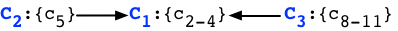
\includegraphics[scale=0.6]{DepDAG.png}
%% \end{figure}
%% \vspace*{-0.08in}
%% Each node (labeled $C_i$) is a set of constraints that belong to a
%% strongly connected component in the dependency graph ($G_c$), hence
%% are mutually dependent. All dependencies, except the self-dependency
%% on $\mathbf{c_{10}}$, are type-2 dependencies.

A dependency DAG makes the dependencies between constraints explicit.
Constraints in each set are mutually dependent, and need to be solved
simultaneously, whereas constraints in different sets can be solved as
per any valid topological ordering of the graph's transpose.
Accordingly, we obtain a topological ordering of nodes in the graph
$G_{{C}}^{T}$ ($G_C$'s transpose), and solve the sets of constraints
in that order. The solutions obtained after solving a constraint set
are applied to the constraints in subsequent sets before attempting to
solve them.  Consequently, when the turn of a constraint set ($C$)
arrives during the constraint solving process, it satisfies certain
properties:
\begin{itemize}
\item There exists only one predicate variable ($\varphi$) that is either
constrained or used by the constraints in the set ($C$). The variable is
called set's \emph{subject}. This property follows from (a). the fact
that all the dependency constraints have already been solved (and
solutions applied), and (b). the assumption that there are no mutually
recursive definitions. 
\item All the constraints that constrain the set's subject are present
in the set. This follows from our definition of the dependency relation.
\end{itemize}

%% For the DAG in figure above, we consider the topological order $[C_1,
%% C_2, C_3]$ of its transpose, and solve the sets of constraints in that
%% order.

\subsection{Expression Elaboration}

\begin{figure}

\begin{codeml}
$\elabExpr(CT, \A, \ralloc, \env, e)$ = 
  match $e$ with
  | $\C{new} \fgjN(\bar{e})$ $\longrightarrow$ 
    let $\fbN$ = $\templateTy(\fgjN)$ in
    let $C_1$ = $\typeOk({\A},{\fbN})$ in
    let $C_2$ = match $\fgjN$ with $\RgnZ\inang{T}$ $\longrightarrow$ $\top$
          | _ $\longrightarrow$ $\{\isvalid{\A.\phicx}{\allocRgn(\fbN)=\ralloc}\}$ in
    let ($\_:\taubar$) = $\fields(\fbN)$
    let $(\bar{e'}:\bar{\tau'}, C_3)$ = $\elabExpr(\A,\ralloc,\env,\bar{e})$ in
    let $C_4$ = $\subtypeOk({\A},{\bar{\tau'}},{\taubar})$ in
      ($\C{new} \fbN(\bar{e'}) : \fbN$,$\bigcup_{i=1}^4 C_i$)
  | $e_a(\bar{e})$ $\longrightarrow$ 
    let ($e_a':\inang{\rhoalloc\rhobar\,|\,\phi}\taubar \xrightarrow{\rgn} \tau$,$C_1$) = 
                $\elabExpr(\A,\ralloc,\env,e_a)$ in
    let $\bar{\rho'}$ = $\bar{\fresh_\rho()}$ in
    let $C_2$ = $\{\bar{\rho'} \in \A.\rhoenv\}$ in
    let $\substFn$ = $[\bar{\rho'}/\rhobar][\ralloc/\rhoalloc]$ in
    let $C_3$ = $\{\isvalid{\A.\phicx}{\substFn(\phi)}\}$ in
%*   %let $(C_3,C_4)$ = $(\typeOk(\substFn(\taubar)), \typeOk(\substFn(\tau)))$ in 
*)   let $(\bar{e'}:\bar{\tau'}, C_4)$ = $\elabExpr(\A,\ralloc,\env,\bar{e})$ in
    let $C_5$ = $\subtypeOk({\A},{\bar{\tau'}},{\bar{\substFn(\tau)}})$ in
      ($e_a'\inang{\ralloc\bar{\rho'}}(\bar{e'}):\substFn(\tau)$,$\bigcup_{i=1}^5 C_i$)
  | $\letregion{\rgn}{e_a}$ $\longrightarrow$
    let $\rgn'$ = $\fresh_{\rgn}()$ in 
    let $(\rhoenv,\aenv,\phicx)$ = $\A$ in
    let $\A'$ = ($\rhoenv \cup \{\rgn'\}, \aenv, \phicx \conj (\rhoenv \outlives \rgn')$) in
    let ($e_a':\tau$,$C_1$) = $\elabExpr(\A',\rgn',\env,[\rgn'/\rgn]e_a)$ in
      ($\letregion{\rgn'}{e_a'}:\tau$,$C_1$)
  | $\open{e_a}{\rgn}{y}{e_b}$ $\longrightarrow$ 
    let ($e_a':\RgnZ\inang{T}\inang{\rho}$,$C_1$) = 
                $\elabExpr(\A,\ralloc,\env,e_a)$ in
    let $\rgn'$ = $\fresh_{\rgn}()$ in 
    let $(\rhoenv,\aenv,\phicx)$ = $\A$ in
    let ($\A'$,$\env'$) = ($(\rhoenv \cup \{\rgn'\},\aenv,\phicx)$,$\env[y\mapsto T@\rgn']$) in
    let ($e_b':\tau$,$C_2$) = $\elabExpr(\A',\rgn',\env',[\rgn'/\rgn]e_a)$ in
      ($\open{e_a'}{\rgn'}{y}{e_b'} : \tau$, $C_1 \cup C_2$)
  | _ $\longrightarrow$ ...
\end{codeml}

\caption{Constraint generation for expressions in $\absof{\FB}$}
\label{fig:fb-elabexpr}
\end{figure}

\newcommand{\hdOf}[2]{\C{class}\; #1\angAlpha\inang{\rhoalloc\rhobar \,|\, #2} \extends \fbN}
\begin{figure}

\begin{codeml}
$\elabMeth(CT, B, \tau \; m\inang{\rhoalloc_m\rhobarm \,|\, \varphi_m} (\taubar \; \xbar)\{\C{return} e;\})$ = 
  let $\hdOf{B}{\varphi}\{\bar{\tau^f}\,\xbar;\;k\;\bar{d}\}$ = $CT(B)$ in
  let ($\rhoenv$,$\aenv$,$\phicx$) as $\A$ = 
            $(\{\rhoalloc,\rhobar,\rhoalloc_m,\rhobarm\},\bar{\tyvar} \extends \bar{\fgjN},\varphi \conj \varphi_m)$ in
  let $C_1$ = $\{\tywf{\rhoenv}{\varphi_m}\}$ in
  let $\env$ = $\cdot[\thisZ \mapsto B\inang{\bar{\tyvar}}\inang{\rhoalloc\rhobar}][\xbar \mapsto \taubar]$ in
  let ($e':\tau'$,$C_2$) = $\elabExpr (\A,\rhoalloc_m,\env,e)$ in
  let $C_3$ = $\subtypeOk({\A},{\tau'},{\tau})$ in
    ($\tau \; m\inang{\rhoalloc_m\rhobarm \,|\, \varphi_m} (\taubar \;
    \xbar)\{\C{return} e';\}$, $C_1 \cup C_2 \cup C_3$)
\end{codeml}

\begin{codeml}
$\elabClass(CT,B)$ = 
  let $\hdOf{B}{\varphi}\{\bar{\tau^f}\,\xbar;\;k\;\bar{d}\}$ = $CT(B)$ in
  let ($\rhoenv$,$\aenv$,$\phicx$) as $\A$ = $(\{\rhoalloc,\rhobar\},\bar{\tyvar} \extends \bar{\fgjN},\varphi)$ in
  let $C_1$ = $\tywf{\rhoenv}{\varphi}$ in
  let ($C_2$,$C_3$) = ($\typeOk({\A},{\fbN})$,$\typeOk({\A},{\bar{\tau^f}})$) in
  let $C_4$ = $\{\isvalid{\phicx}{\allocRgn(\bar{\tau^f}) \outlives \rhoalloc \conj \allocRgn(\fbN) = \rhoalloc}\}$ in
  let ($k'$,$C_5$) = $\elabCons(B,k)$ in
  let ($\bar{d'}$,$C_6$) = $\elabMeth(B,\bar{d})$ in
    ($\hdOf{B}{\varphi}\{\bar{\tau^f}\,\xbar;\;k'\;\bar{d'}\}$, $\bigcup_{i=1}^6 C_i$)
\end{codeml}
%
% \begin{codeml}
% $\elabClassTable(CT)$ = 
%   let ($CT'$,$C$) = (ref $\cdot$, ref $\emptyset$) in
%   let _ = foreach $B \in dom(CT)$ do
%             let ($D_B$,$C_B$) = $\elabClass(CT,B)$ in
%               $CT'$ := $CT'[B \mapsto D_B]$;
%               $C$ := $C \cup C_B$
%            done in
%   let ($\substFn_\rho$,$\substFn_\varphi$) = $\solve(C)$ in
%     $\substFn_\varphi(\substFn_\rho(CT')) $
%       
% \end{codeml}

\caption{Method, class and class table elaboration}
\label{fig:fb-elabmeth}
\end{figure}


%Elaborating $\absof{\FB}$ expressions to $\FB$ expressions involves
%(a). replacing core types in variable declarations and \C{new}
%expressions with fresh region type templates, and (b). explicitly
%instantiating region parameters of methods with fresh region variables
%in method calls and function applications. This elaboration is
%performed with respect to the polymorphic type templates of classes
%and methods computed as per \S\ref{sec:fb-templatization}. 

Function $\elabExpr$, shown in Fig.~\ref{fig:fb-elabexpr}, performs
this elaboration for a subset of expressions in $\absof{\FB}$, whose
corresponding $\FB$ expressions have been ascribed static semantics in
Fig.~\ref{fig:fb-staticsem}. $\elabExpr$ is defined under the same
context as the expression typing judgment in
Fig.~\ref{fig:fb-staticsem} with symbols $\A$,$\ralloc$, and $\env$
retaining their meaning. The function traverses expressions in a
syntax-directed manner of a type checker, introducing fresh region
type templates for unknown region types, while generating constraints
over region and predicate variables. The precise nature of generated
constraints is explained in \S\ref{sec:fb-constraintsem}, but in
summary, they capture the relationships between the type templates of
various subexpressions and their well-formedness. Note that
$\elabExpr$ returns the region type template of the subexpression,
which is used to generate constraints for the expression. Functions
$\typeOk$ and $\subtypeOk$ (definitions not shown) used by $\elabExpr$
implement type well-formedness and subtype judgments from
Fig.~\ref{fig:fb-staticsem}, respectively.

\subsection{Method and Class Elaboration}

Functions $\elabMeth$ and $\elabClass$ shown in
Fig.~\ref{fig:fb-elabmeth} lift expression elaboration to method and
class definitions, respectively. Both functions first build a context
($\A$) containing a set ($ \rhoenv$) of region variables denoting
regions that are currently live, a map ($\aenv$) mapping type
variables to their bounds, and a constraint formula ($\phicx$)
capturing constraints over live region variables. We use predicate
variables ($\varphi$ and $\varphi_m$) to capture constraints over
variables in $\rhoenv$ denoting the fact that such constraints are yet
to be inferred.

Function $\elabMeth$ elaborates a method definition of class $B$. It
calls $\elabExpr$ with the context $\A$, its allocation context
parameter ($\rhoallocm$), and a type environment ($\env$) that
contains region type bindings for all the arguments of the method,
including the implicit $\C{this}$ argument. The region type template
returned by $\elabExpr$ for the method body is checked against its
expected type (derived from the type template of the method)
generating more constraints. The function then returns the elaborated
method definition and the set of constraints.

$\elabClass$ elaborates the definition of a class $B$. It relies on
$\elabCons$\footnote{The definition of $\elabCons$ is straightforward,
hence not shown.} and $\elabMeth$ functions to elaborate $B$'s
constructor ($k$) and method definitions ($\bar{d}$), respectively. To
the set of constraints returned by these functions, $\elabClass$ adds
constraints generated by checking the well-formedness of the type
templates of its superclass and fields, and also a new constraint
capturing a couple of safety conditions: first, the allocation regions
of objects referred by the instance variables should outlive the
allocation region of the instance itself, and second, the allocation
regions of a class type and its superclass type must be the same.

Function $\elabClassTable$ (Fig.~\ref{fig:fb-elabmeth}) elaborates
every definition in the class table $CT$, while accumulating
constraints.
